\documentclass[a4paper,12pt]{report}
\usepackage{graphicx}
\title{Tugas pemrograman Cahapter 3}
\author{Nuha Hanifatul Khonsa'}
\date{1 Desember 2019}
\begin{document}


\maketitle


\section{Teori}
\subsection{Fungsi}
\par Fungsi adalah blok kode terorganisir dan dapat digunakan kembali yang digunakan untuk melakukan sebuah tindakan/action. Fungsi memberikan modularitas yang lebih baik untuk aplikasi Anda dan tingkat penggunaan kode yang tinggi. Fungsi blok dimulai dengan def kata kunci diikuti oleh nama fungsi dan tanda kurung (()).

Contoh fungsi sederhana:
    \begin{center}
    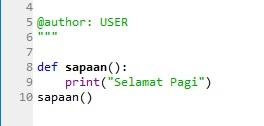
\includegraphics[width=11cm\textwidth]{Figure/fungsi1.jpg}
    \end{center}
Fungsi dengan pengembalian nilai
    \begin{center}
    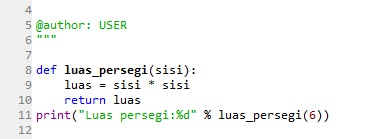
\includegraphics[width=11cm\textwidth]{Figure/fungsi2.jpg}
    \end{center}
    
\subsection{Package}
\par  Package sebagaik pengelompokkan atau pengorganisasian modul yang telah dibuat. seperti halnya  kita tidak perlu membuat script untuk beberapa kasus, namun kita bisa mengemasnya dalam 1 file tiap kasus dan bisa memanggil file tersebut dalam 1 program.

Cara memanggil Package ialah:
\begin{center}
    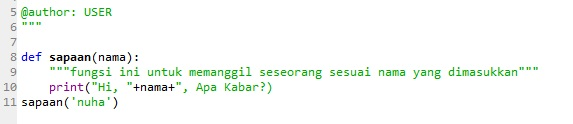
\includegraphics[width=11cm\textwidth]{Figure/package.jpg}
    \end{center}
    
\subsection{Class}
\par Blueprint dari sebuah object yang akan dibangun yang mendefinisikan seperangkat atribut yang menjadi ciri dari object class tersebut.
    \begin{center}
    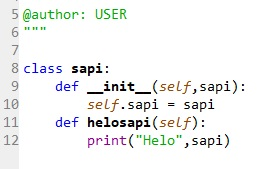
\includegraphics[width=11cm\textwidth]{Figure/class.jpg}
    \end{center}
    
\subsection{Object}
\par Bagian program yang berada dalam sebuah class yang memiliki suatu variable yang saling berhubungan.
    \begin{center}
    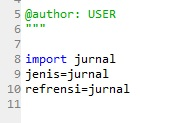
\includegraphics[width=11cm\textwidth]{Figure/obcjact.jpg}
    \end{center}
    
\subsection{Atribute}
\par Tempat menampung data maupun perintah pada object dalam sebuah kelas.
    \begin{center}
    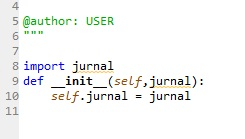
\includegraphics[width=11cm\textwidth]{Figure/atribut.jpg}
    \end{center}

\subsection{Method}
\par Method merupakan sebuah fungsi yang berada dalam suatu class
    \begin{center}
    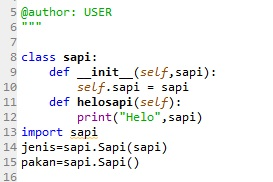
\includegraphics[width=11cm\textwidth]{Figure/methode.jpg}
    \end{center}
    
\subsection{Contoh Penggunaan Library}
    \begin{center}
    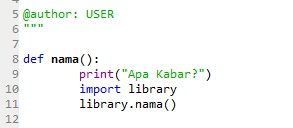
\includegraphics[width=11cm\textwidth]{Figure/library.jpg}
    \end{center}
    
\subsection{Penggunaan Package From Kalkulator Import}
\par Hal pertama yang dapat kita lakukan ialah membuat package perhitungan. Package perhitungan ini yang nantinya akan diimport.
    \begin{center}
    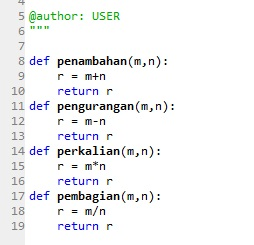
\includegraphics[width=11cm\textwidth]{Figure/kalkulator.jpg}
    \end{center}
\par Lalu import package perhitungan tadi seperti:
    \begin{center}
    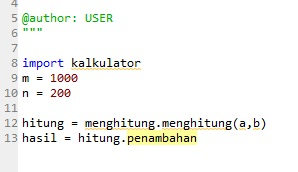
\includegraphics[width=11cm\textwidth]{Figure/kalkulatorim.jpg}
    \end{center}
    
\subsection{Pemanggilan Library dalam Sebuah Folder}
\par Untuk dapat memanggil sebuah library dalam sebuah folder yang pertama-tama yang harus dilakukan ialah, memanggil nama foldernya terlebih dahulu lalu dilanjutkan dengan mengimport
library seperti ini :
    \begin{center}
    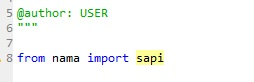
\includegraphics[width=11cm\textwidth]{Figure/libfolder.jpg}
    \end{center}

\subsection{Pemanggilan Class dalam Sebuah Folder}
\par Saat akan memanggil sebuah class yang pertama-tama yang harus dilakukan ialah memanggil  folder.
Kita dapat menuliskan nama folder lalu dilanjutkan dengan mengimport nama class
nya, seperti ini :
    \begin{center}
    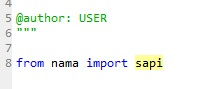
\includegraphics[width=11cm\textwidth]{Figure/clasfolder.jpg}
    \end{center}
    
\section{Ketrampilan Pemrograman}
\item Soal 1
    \begin{center}
    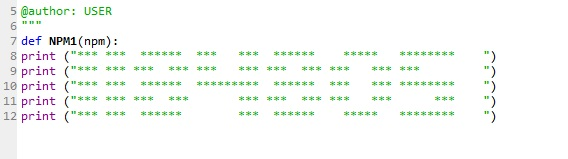
\includegraphics[width=11cm\textwidth]{Ketrampilan/1.jpg}
    \end{center}
\item Soal 2
    \begin{center}
    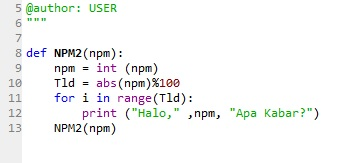
\includegraphics[width=11cm\textwidth]{Ketrampilan/2.jpg}
    \end{center}
\item Soal 3
    \begin{center}
    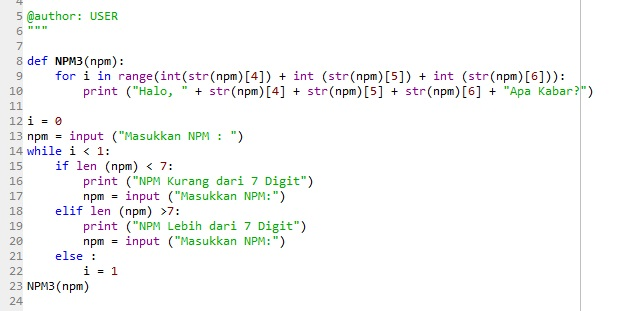
\includegraphics[width=11cm\textwidth]{Ketrampilan/3.jpg}
    \end{center}
\item Soal 4
    \begin{center}
    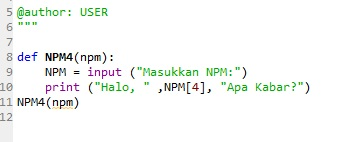
\includegraphics[width=11cm\textwidth]{Ketrampilan/4.jpg}
    \end{center}
\item Soal 5
    \begin{center}
    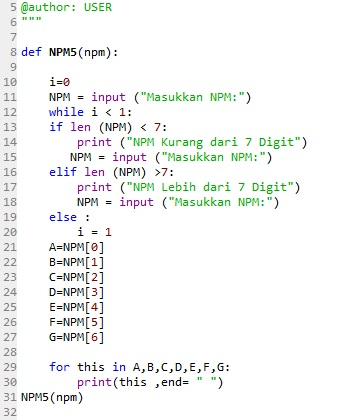
\includegraphics[width=11cm\textwidth]{Ketrampilan/5.jpg}
    \end{center}
\item Soal 6
    \begin{center}
    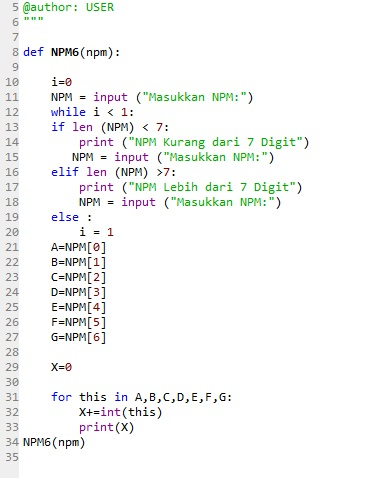
\includegraphics[width=11cm\textwidth]{Ketrampilan/6.jpg}
    \end{center}
\item Soal 7
    \begin{center}
    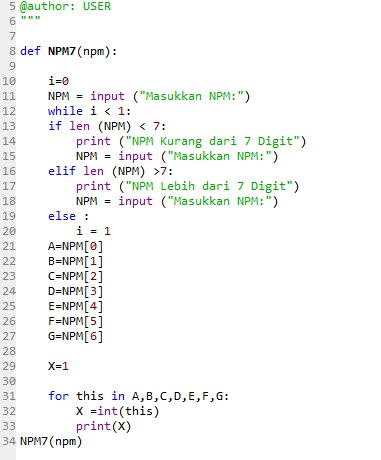
\includegraphics[width=11cm\textwidth]{Ketrampilan/7.jpg}
    \end{center}
\item Soal 8
    \begin{center}
    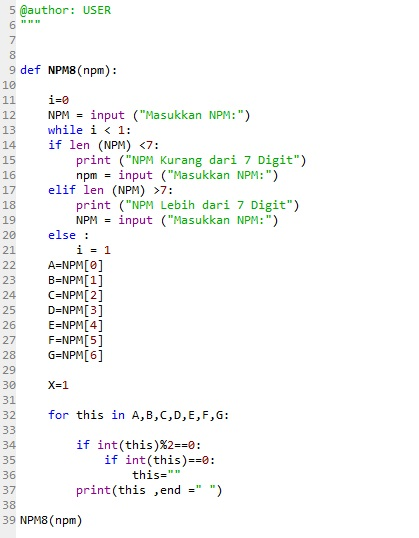
\includegraphics[width=11cm\textwidth]{Ketrampilan/8.jpg}
    \end{center}
\item Soal 9
    \begin{center}
    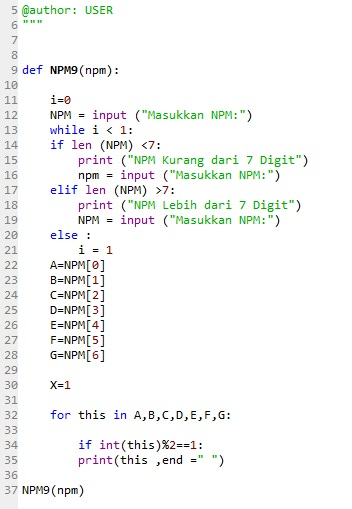
\includegraphics[width=11cm\textwidth]{Ketrampilan/9.jpg}
    \end{center}
\item Soal 10
    \begin{center}
    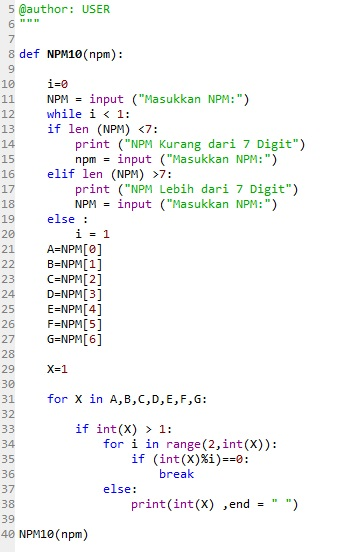
\includegraphics[width=11cm\textwidth]{Ketrampilan/10.jpg}
    \end{center}

\end{document}
